\clearpage
\cleardoublepage

\chapter{训练过程与框架}

\section{引言}

训练神经网络是找到使给定损失函数在数据集上最小化的参数集的过程。虽然优化的数学基础（梯度下降、反向传播）已在前面章节介绍，但本章聚焦于训练过程本身的\textbf{实践和理论方面}。我们探讨为什么某些技术有效、如何诊断训练失败，以及现代框架如何使大规模训练变得可行。

训练过程涵盖多个相互关联的组成部分：优化算法、正则化策略、超参数配置以及高效计算的基础设施。深入理解这些组成部分如何相互作用对于成功训练现代神经网络至关重要。

\section{训练循环}

神经网络训练包括使用小批量随机梯度下降（SGD）或其变体对数据进行迭代优化。

\subsection{形式化描述}

给定数据集$\mathcal{D} = \{(\mathbf{x}_i, \mathbf{y}_i)\}_{i=1}^{N}$、模型$f(\mathbf{x}; \theta)$（参数为$\theta$）和损失函数$\ell$，训练目标是：
\begin{equation}
\theta^* = \arg\min_{\theta} \frac{1}{N}\sum_{i=1}^{N} \ell\bigl(f(\mathbf{x}_i; \theta), \mathbf{y}_i\bigr)
\end{equation}

实际上，我们对大小为$B$的小批量$\mathcal{B}_t \subset \mathcal{D}$计算梯度：
\begin{equation}
\mathbf{g}_t = \nabla_\theta \frac{1}{B}\sum_{i \in \mathcal{B}_t} \ell\bigl(f(\mathbf{x}_i; \theta_t), \mathbf{y}_i\bigr)
\end{equation}

\begin{algorithm}[H]
\caption{训练循环}
\begin{enumerate}
    \item 初始化模型权重$\theta_0$
    \item 对于每个轮次$e = 1, 2, \ldots, E$：
    \begin{enumerate}
        \item 打乱训练数据
        \item 对于每个小批量$\mathcal{B}_t$：
        \begin{enumerate}
            \item 前向传播：计算预测$\hat{\mathbf{y}} = f(\mathbf{x}; \theta_t)$
            \item 计算损失$\mathcal{L}_t = \frac{1}{B}\sum_{i \in \mathcal{B}_t} \ell(\hat{\mathbf{y}}_i, \mathbf{y}_i)$
            \item 反向传播：计算梯度$\mathbf{g}_t = \nabla_\theta \mathcal{L}_t$
            \item 更新权重：$\theta_{t+1} = \theta_t - \alpha \cdot \text{optimizer\_step}(\mathbf{g}_t)$
        \end{enumerate}
        \item 在验证集上评估
        \item 如果验证指标改进则保存检查点
    \end{enumerate}
    \item 返回最佳模型
\end{enumerate}
\end{algorithm}

\subsection{为什么小批量SGD有效}

一个自然的问题是：为什么要使用小批量而不是在整个数据集上计算精确梯度？答案在于三个因素之间的有益相互作用：

\begin{enumerate}
    \item \textbf{噪声作为隐式正则化。}小批量的梯度噪声防止优化器陷入泛化能力差的尖锐最小值。Keskar等人 \cite{keskar2017largebatch}表明，大批量训练倾向于收敛到"尖锐"最小值，泛化能力较差，而小批量SGD找到"平坦"最小值。
    
    \item \textbf{计算效率。}现代硬件（GPU/TPU）针对并行矩阵运算进行了优化。批次大小32-256可以充分利用GPU并行性，同时仍提供有意义的梯度估计。
    
    \item \textbf{定期进度监控。}每个小批量步骤都提供一个信号，允许在浪费数小时计算之前早期检测训练问题（发散、振荡）。
\end{enumerate}

\begin{theorem}[SGD在递减学习率下的收敛性]
在$\mathcal{L}$的凸性和平滑性假设下，学习率调度$\alpha_t = \mathcal{O}(1/\sqrt{t})$的SGD满足：
\begin{equation}
\mathbb{E}[\mathcal{L}(\theta_T)] - \mathcal{L}(\theta^*) \leq \mathcal{O}\!\left(\frac{1}{\sqrt{T}}\right)
\end{equation}
相比之下，完整批次梯度下降为$\mathcal{O}(1/T)$。较慢的速率是为每步更便宜计算付出的代价。
\end{theorem}

\section{超参数}

影响训练动态和最终模型质量的关键超参数。

\subsection{学习率}

学习率$\alpha$可以说是最重要的超参数。它直接控制参数空间中的步长，并决定训练是收敛、振荡还是发散。

\subsubsection{学习率的影响}

\begin{itemize}
    \item \textbf{太高：}损失发散或剧烈振荡。优化器"越过"最小值。
    \item \textbf{太低：}训练收敛极慢，可能被困在较差的局部最小值或鞍点。
    \item \textbf{适中：}损失稳定下降，有轻微振荡提供正则化。
    \item \textbf{典型范围：} $10^{-5}$到$0.1$
    \item \textbf{Adam默认值：} $10^{-3}$
    \item \textbf{SGD默认值：} $10^{-2}$
\end{itemize}

\subsubsection{学习率范围测试}

Smith \cite{smith2017cyclical}提出了一种简单但有效的寻找良好学习率的方法。思路是在单次训练运行中从非常小的学习率指数增长到很大的值，绘制损失与学习率的关系图：

\begin{enumerate}
    \item 从$\alpha_{\min} = 10^{-6}$（或更小）开始
    \item 每个批次将$\alpha$增加$e$因子（或常数因子）
    \item 当损失开始增加时停止
    \item 选择最陡下降点的$\alpha$（通常为最大值的$10^{-1}$到$10^{-1}$）
\end{enumerate}

\begin{figure}[htbp]
    \centering
    \begin{tikzpicture}[scale=0.9]
        \draw[->] (0,0) -- (10,0) node[right] {Learning rate ($\log$ scale)};
        \draw[->] (0,0) -- (0,5) node[above] {Loss};
        % Loss curve
        \draw[thick, blue] plot[smooth] coordinates {
            (0.5, 4.5) (1, 3.8) (1.5, 3.0) (2, 2.3) (2.5, 1.8) 
            (3, 1.5) (3.5, 1.3) (4, 1.2) (4.5, 1.15) (5, 1.1)
            (5.5, 1.2) (6, 1.5) (6.5, 2.0) (7, 3.0) (7.5, 4.5)
        };
        % Steepest descent point
        \draw[dashed, red] (4, 1.2) -- (4, 0) node[below] {\small $\alpha^*$};
        \draw[dashed, red] (4, 1.2) -- (0, 1.2);
        \draw[->, red, thick] (1.5, 3.0) -- (2.3, 2.2);
        \node[red, right] at (2.3, 2.5) {\small Steepest descent};
        % Labels
        \node[blue, right] at (7.5, 4.5) {\small Divergence};
        \node at (-0.3, 5) {\small High};
        \node at (-0.3, 0) {\small Low};
    \end{tikzpicture}
    \caption[学习率范围测试]{学习率范围测试。最陡下降点$\alpha^*$提供了良好的初始学习率。}
    \label{fig:lr_range_test}
\end{figure}

\subsubsection{学习率预热}

对于使用Adam训练的大型模型，标准做法是使用预热阶段，在前几百或几千步内将学习率从零逐渐增加到目标值。这可以防止在Adam动量估计不可靠的早期阶段（初始化为零时）出现不稳定。

预热调度通常是：
\begin{equation}
\alpha_t = \alpha_{\max} \cdot \min\!\left(1, \frac{t}{T_{\text{warmup}}}\right)
\end{equation}
其中$T_{\text{warmup}}$是预热步数（例如，Transformer模型 \cite{vaswani2017attention}为1000）。

\subsection{批次大小}

批次大小$B$控制每次参数更新前处理的样本数。它对训练速度和模型质量都有深远影响。

\subsubsection{批次大小的影响}

\begin{itemize}
    \item \textbf{小批次（16-64）：}噪声更大的梯度提供隐式正则化，通常泛化能力更好。但GPU并行性利用不足。
    \item \textbf{中等批次（64-256）：}泛化和硬件利用之间的良好权衡。大多数从业者的默认选择。
    \item \textbf{大批次（256-8192+）：}更好的硬件利用率，更快的时钟训练。但通常需要学习率缩放，可能损害泛化能力。
\end{itemize}

\subsubsection{线性缩放规则}

Goyal等人 \cite{goyal2017accurate}提出了大批次训练的线性缩放规则：当批次大小乘以$k$时，学习率也应乘以$k$：
\begin{equation}
\alpha_{\text{large}} = \alpha_{\text{small}} \times \frac{B_{\text{large}}}{B_{\text{small}}}
\end{equation}

\begin{note}[批次大小与泛化]
Keskar等人 \cite{keskar2017largebatch}和Hoffer等人 \cite{hoffer2017train}的研究表明，较小的批次通常获得更好的泛化能力，因为梯度噪声起到隐式正则化的作用。然而，效果取决于学习率、网络架构和训练时长等其他因素。
\end{note}

\begin{table}[ht]
    \centering
    \caption{超参数范围和默认值}
    \begin{tabular}{L{2.8cm} L{3cm} L{3.5cm} L{3cm}}
        \toprule
        \textbf{超参数} & \textbf{典型范围} & \textbf{默认值} & \textbf{备注} \\
        \midrule
        学习率 & $10^{-5}$ 到 $0.1$ & Adam: $10^{-3}$；SGD: $10^{-2}$ & 最重要 \\
        批次大小 & 16-8192 & 32-256 & 取决于GPU内存 \\
        训练轮次 & 10-1000 & 任务相关 & 推荐使用早停 \\
        权重衰减 & $10^{-6}$ 到 $10^{-2}$ & $10^{-2}$（AdamW） & 见第~\ref{sec:weight_decay}节 \\
        Dropout率 & 0.1-0.5 & 0.1-0.3 & 见第~\ref{sec:dropout_theory}节 \\
        动量 & 0.9-0.999 & 0.9（SGD） & Adam为0.9/0.999 \\
        预热步数 & 0-10K & 1000（Transformers） & 大模型受益更多 \\
        \bottomrule
    \end{tabular}
\end{table}

\section{正则化}

正则化包括所有通过约束模型容量或向训练过程添加噪声来减少过拟合的技术。我们为最重要的方法提供理论基础。

\subsection{Dropout}
\label{sec:dropout_theory}

Dropout \cite{srivastava2014dropout}是一种正则化技术，在训练期间以概率$p$（dropout率）随机将神经元激活置零。

\subsubsection{带Dropout的前向传播}

对于输入$\mathbf{x}$和权重矩阵$\mathbf{W}$的层，在训练期间：
\begin{equation}
\mathbf{y} = \mathbf{W} \cdot (\mathbf{x} \odot \mathbf{m}), \quad \mathbf{m} \sim \text{Bernoulli}(1 - p)
\end{equation}
其中$\mathbf{m}$是二进制掩码，$\odot$表示逐元素乘法。

\subsubsection{反转Dropout}

标准实现使用\textbf{反转Dropout}，在训练期间缩放激活，以便在推理时不需要缩放：
\begin{equation}
\mathbf{y} = \frac{\mathbf{W} \cdot (\mathbf{x} \odot \mathbf{m})}{1 - p}
\end{equation}

这确保了$\mathbb{E}[\mathbf{y}_{\text{train}}] = \mathbf{W}\mathbf{x} = \mathbf{y}_{\text{inference}}$，意味着有无dropout的期望输出相同。

\textbf{证明：}对于输入的任意分量$x_j$：
\begin{align}
\mathbb{E}\left[\frac{x_j \cdot m_j}{1 - p}\right] &= \frac{1}{1-p} \cdot \mathbb{E}[x_j \cdot m_j] \\
&= \frac{1}{1-p} \cdot x_j \cdot \mathbb{E}[m_j] \\
&= \frac{1}{1-p} \cdot x_j \cdot (1 - p) = x_j
\end{align}

\subsubsection{集成解释}

Dropout可以理解为训练$2^n$个共享参数的子网络集成（其中$n$是dropout单元数）。每次前向传播使用不同的掩码有效地对不同的子网络进行采样。在推理时，所有子网络被平均（根据缩放的线性性质，这等价于使用完整网络）。

更准确地说，具有$n$个dropout单元的网络有$2^n$个可能的精简网络。Dropout训练目标最小化：
\begin{equation}
\mathcal{L}_{\text{dropout}} = \mathbb{E}_{\mathbf{m} \sim \text{Bernoulli}(1-p)} \left[\ell\bigl(f(\mathbf{x}; \theta \odot \mathbf{m}), \mathbf{y}\bigr)\right]
\end{equation}

这等价于最小化\textbf{装袋集成}目标，解释了Dropout通过方差减少的正则化效果。

\subsubsection{Dropout作为近似贝叶斯推理}

Gal和Ghahramani \cite{gal2016dropout}表明，神经网络中的Dropout在数学上等价于深度高斯过程中的近似变分推理。在这个解释下：
\begin{itemize}
    \item 每个dropout掩码定义了来自近似后验$q(\theta)$的样本
    \item 隐式地最小化近似后验和真实后验之间的KL散度
    \item 推理时多次随机前向传播提供不确定性估计
\end{itemize}

这为Dropout不仅提供正则化而且提供\textbf{模型不确定性}估计的原则性解释——这是安全关键应用的关键特性。

\subsubsection{Dropout变体}

\begin{table}[ht]
    \centering
    \caption{Dropout变体及其特性}
    \begin{tabular}{L{3cm} L{4cm} L{4cm}}
        \toprule
        \textbf{变体} & \textbf{机制} & \textbf{使用场景} \\
        \midrule
        标准Dropout & 随机将激活置零 & 全连接层 \\
        空间Dropout & 将整个特征图置零 & 卷积层 \\
        DropConnect & 随机将权重置零 & Dropout的替代 \\
        DropBlock & 将连续区域置零 & 卷积层 \\
        注意力Dropout & 将注意力权重置零 & Transformer模型 \\
        特征Dropout & 将输入特征置零 & 输入正则化 \\
        \bottomrule
    \end{tabular}
\end{table}

\subsection{权重衰减}
\label{sec:weight_decay}

\subsubsection{L2正则化作为MAP估计}

权重衰减（L2正则化）对模型参数的大小添加惩罚：
\begin{equation}
\mathcal{L}_{\text{reg}} = \mathcal{L} + \frac{\lambda}{2}\|\mathbf{W}\|_F^2
\end{equation}

这作为\textbf{最大后验}（MAP）估计有着优雅的解释。假设权重$\mathbf{W} \sim \mathcal{N}(0, \sigma_w^2 \mathbf{I})$的高斯先验。MAP目标是：
\begin{align}
\theta_{\text{MAP}} &= \arg\max_\theta \log p(\mathcal{D} | \theta) + \log p(\theta) \\
&= \arg\min_\theta \underbrace{-\sum_{i=1}^N \log p(\mathbf{y}_i | \mathbf{x}_i, \theta)}_{\mathcal{L}} + \underbrace{\frac{1}{2\sigma_w^2}\|\mathbf{W}\|_F^2}_{\lambda/2 \cdot \|\mathbf{W}\|_F^2}
\end{align}

因此，系数为$\lambda$的L2正则化等价于方差为$\sigma_w^2 = 1/\lambda$的高斯权重先验的MAP估计。

\subsubsection{权重衰减 vs. L2正则化：AdamW}

对于Adam等自适应优化器，L2正则化和解耦权重衰减之间存在微妙但重要的区别。在带L2正则化的标准Adam中，权重更新变为：
\begin{equation}
\mathbf{W}_{t+1} = \mathbf{W}_t - \alpha \cdot \frac{\hat{\mathbf{m}}_t}{\sqrt{\hat{\mathbf{v}}_t} + \epsilon} \odot \left(\nabla \mathcal{L}_t + \lambda \mathbf{W}_t\right)
\end{equation}

问题是权重衰减项$\lambda \mathbf{W}_t$被自适应学习率$\frac{1}{\sqrt{\hat{\mathbf{v}}_t} + \epsilon}$缩放，意味着具有大历史梯度的参数接收\textbf{较少}的正则化——这与我们想要的相反。

Loshchilov和Hutter \cite{loshchilov2019decoupled}提出了\textbf{AdamW}，将权重衰减与基于梯度的更新解耦：
\begin{align}
\mathbf{W}_{t+1} &= \mathbf{W}_t - \alpha \cdot \frac{\hat{\mathbf{m}}_t}{\sqrt{\hat{\mathbf{v}}_t} + \epsilon} \odot \nabla \mathcal{L}_t - \alpha\lambda \mathbf{W}_t \\
&= (1 - \alpha\lambda)\mathbf{W}_t - \alpha \cdot \frac{\hat{\mathbf{m}}_t}{\sqrt{\hat{\mathbf{v}}_t} + \epsilon} \odot \nabla \mathcal{L}_t
\end{align}

这确保了权重衰减均匀应用，无论自适应学习率如何，在实践中导致明显更好的泛化能力。

\subsection{其他正则化技术}

\subsubsection{梯度裁剪}

对于训练非常深的网络或循环网络，梯度可能变得非常大，导致使训练不稳定的参数更新。梯度裁剪限制梯度范数：
\begin{equation}
\text{若 } \|\mathbf{g}\| > c: \quad \mathbf{g} \leftarrow \frac{c}{\|\mathbf{g}\|}\mathbf{g}
\end{equation}

其中$c$是阈值（Transformer模型通常为1.0或5.0）。Pascanu等人 \cite{pascanu2013difficulty}表明，梯度裁剪对于在长序列上训练RNN至关重要。

\subsubsection{标签平滑}

标签平滑 \cite{szegedy2016rethinking}用更软的分布替换硬独热标签。不是目标$\mathbf{y} = [0, \ldots, 0, 1, 0, \ldots, 0]$，而是使用：
\begin{equation}
y_k^{\text{smooth}} = (1 - \epsilon)\cdot y_k + \frac{\epsilon}{K}
\end{equation}
其中$\epsilon$是平滑系数（通常为0.1），$K$是类别数。

\textbf{标签平滑有效的原因：}它防止模型变得过于自信。在训练数据上输出$p(\text{correct}) = 0.999$的模型可能是在记忆而非学习。标签平滑通过要求模型将一些概率质量分配给不正确的类别来惩罚这一点，这：
\begin{itemize}
    \item 改善校准（预测概率更好地反映真实准确性）
    \item 起到隐式正则化的作用；\cite{muller2019when}将其与输出分布和均匀先验之间的KL散度添加联系起来
    \item 在机器翻译中将BLEU分数提高0.5-1.0
\end{itemize}

\subsubsection{随机深度}

Huang等人 \cite{huang2016deep}提出在训练期间随机丢弃整个残差块（类似于dropout但应用于块级别）。这允许通过减少训练期间的有效深度来训练非常深的网络（例如1200层）：
\begin{equation}
\mathbf{y} = \begin{cases} \mathcal{F}_l(\mathbf{x}) + \mathbf{x} & \text{概率为 } p_l \\ \mathbf{x} & \text{概率为 } 1 - p_l \end{cases}
\end{equation}
其中$p_l$是层$l$的存活概率，通常遵循从第一层到最后一层的线性衰减调度。

\section{早停}

当验证性能停止改进时，早停会停止训练。尽管简单，它是世界上最有效和广泛使用的正则化技术之一。

\subsection{算法}

\begin{enumerate}
    \item 在每个轮次结束时监控验证损失（或合适的指标）
    \item 每当验证指标改进时保存模型检查点
    \item 如果连续$N$个轮次没有观察到改进（\textbf{耐心值}），停止训练
    \item 返回最佳检查点（不是最终的）
\end{enumerate}

典型耐心值：小模型10-20个轮次，大模型5-10个轮次。

\subsection{早停作为正则化}

Yao等人表明，在某些条件下，早停提供的正则化效果等价于权重衰减。直觉很清晰：

\begin{enumerate}
    \item 轮次$t$的模型具有沿优化轨迹的 参数$\theta_t$
    \item 随着训练进展，模型拟合训练数据中越来越细粒度的模式
    \item 超过某一点后，这些模式是噪声（过拟合）
    \item 早停选择参数处于"最佳点"的模型，此时模型已学习信号但尚未学习噪声
\end{enumerate}

形式上，对于具有二次损失的线性模型上的梯度下降，早停等价于Tikhonov正则化（L2权重衰减），其中梯度步数扮演正则化强度的角色。

\section{反向传播}

\subsection{计算图视角}

反向传播是通过以反向拓扑顺序应用链式法则，高效计算通过计算图的梯度的算法。虽然数学原理很简单——链式法则——但计算效率来自于重用中间结果。

\subsubsection{前向传播}

考虑一个简单计算：$z = f(g(x))$。前向传播计算：
\begin{align}
a &= g(x) \\
z &= f(a)
\end{align}

\subsubsection{反向传播}

反向传播以反向顺序计算梯度：
\begin{align}
\frac{\partial \mathcal{L}}{\partial a} &= \frac{\partial \mathcal{L}}{\partial z} \cdot \frac{\partial z}{\partial a} = \frac{\partial \mathcal{L}}{\partial z} \cdot f'(a) \\
\frac{\partial \mathcal{L}}{\partial x} &= \frac{\partial \mathcal{L}}{\partial a} \cdot \frac{\partial a}{\partial x} = \frac{\partial \mathcal{L}}{\partial a} \cdot g'(x)
\end{align}

\subsection{示例：双层网络}

对于具有损失$\mathcal{L}$的双层网络：
\begin{align}
\mathbf{h} &= \sigma(\mathbf{W}_1 \mathbf{x} + \mathbf{b}_1) \\
\hat{\mathbf{y}} &= \mathbf{W}_2 \mathbf{h} + \mathbf{b}_2 \\
\mathcal{L} &= \ell(\hat{\mathbf{y}}, \mathbf{y})
\end{align}

\begin{figure}[htbp]
    \centering
    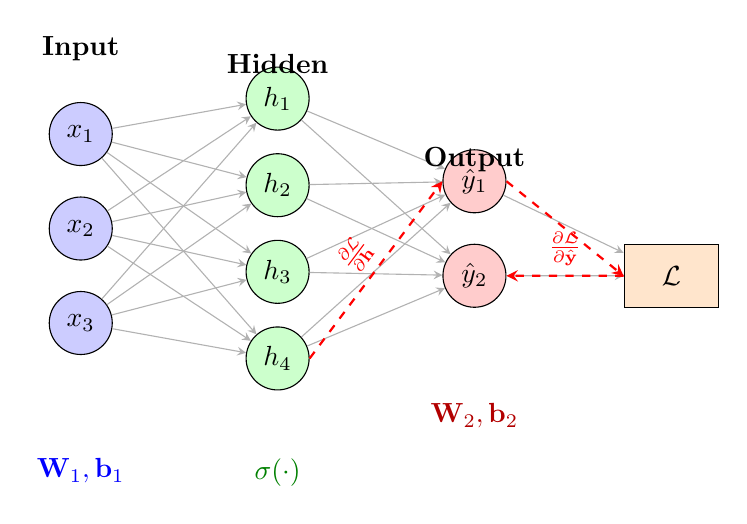
\begin{tikzpicture}[
        node distance=1.5cm,
        neuron/.style={circle, draw, minimum size=8mm, inner sep=0pt},
        >=stealth
    ]
        % Input layer
        \foreach \i in {1,2,3} {
            \node[neuron, fill=blue!20] (I\i) at (0, -\i*1.2+2.4) {$x_{\i}$};
        }
        % Hidden layer
        \foreach \j in {1,2,3,4} {
            \node[neuron, fill=green!20] (H\j) at (2.5, -\j*1.1+2.75) {$h_{\j}$};
        }
        % Output layer
        \foreach \k in {1,2} {
            \node[neuron, fill=red!20] (O\k) at (5, -\k*1.2+1.8) {$\hat{y}_{\k}$};
        }
        % Loss
        \node[rectangle, draw, fill=orange!20, minimum width=1.2cm, minimum height=8mm] (L) at (7.5, -0.6) {$\mathcal{L}$};
        
        % Forward connections
        \foreach \i in {1,2,3} {
            \foreach \j in {1,2,3,4} {
                \draw[->, thin, gray!60] (I\i) -- (H\j);
            }
        }
        \foreach \j in {1,2,3,4} {
            \foreach \k in {1,2} {
                \draw[->, thin, gray!60] (H\j) -- (O\k);
            }
        }
        \foreach \k in {1,2} {
            \draw[->, thin, gray!60] (O\k) -- (L);
        }
        
        % Backward gradient arrows (red, dashed)
        \draw[->, thick, red, dashed] (L.west) -- node[above, font=\small] {$\frac{\partial \mathcal{L}}{\partial \hat{\mathbf{y}}}$} (O2.east);
        \draw[->, thick, red, dashed] (O1.east) -- (L.west);
        \draw[->, thick, red, dashed] (H4.east) -- node[above, font=\small, sloped] {$\frac{\partial \mathcal{L}}{\partial \mathbf{h}}$} (O1.west);
        
        % Labels
        \node[above] at (0, 2.0) {\textbf{Input}};
        \node[above] at (2.5, 1.85) {\textbf{Hidden}};
        \node[above] at (5, 0.6) {\textbf{Output}};
        
        % Layer labels
        \node[below, blue] at (0, -2.8) {$\mathbf{W}_1, \mathbf{b}_1$};
        \node[below, green!50!black] at (2.5, -2.8) {$\sigma(\cdot)$};
        \node[below, red!70!black] at (5, -2.1) {$\mathbf{W}_2, \mathbf{b}_2$};
    \end{tikzpicture}
    \caption{双层网络的计算图。实线箭头表示前向计算；红色虚线箭头表示反向梯度流。}
    \label{fig:computational_graph}
\end{figure}

反向传播计算：
\begin{align}
\frac{\partial \mathcal{L}}{\partial \hat{\mathbf{y}}} &= \nabla_{\hat{\mathbf{y}}} \ell \\
\frac{\partial \mathcal{L}}{\partial \mathbf{W}_2} &= \frac{\partial \mathcal{L}}{\partial \hat{\mathbf{y}}} \mathbf{h}^\top, \qquad \frac{\partial \mathcal{L}}{\partial \mathbf{b}_2} = \frac{\partial \mathcal{L}}{\partial \hat{\mathbf{y}}} \\
\frac{\partial \mathcal{L}}{\partial \mathbf{h}} &= \mathbf{W}_2^\top \frac{\partial \mathcal{L}}{\partial \hat{\mathbf{y}}} \\
\frac{\partial \mathcal{L}}{\partial \mathbf{a}} &= \frac{\partial \mathcal{L}}{\partial \mathbf{h}} \odot \sigma'(\mathbf{a}) \\
\frac{\partial \mathcal{L}}{\partial \mathbf{W}_1} &= \frac{\partial \mathcal{L}}{\partial \mathbf{a}} \mathbf{x}^\top, \qquad \frac{\partial \mathcal{L}}{\partial \mathbf{b}_1} = \frac{\partial \mathcal{L}}{\partial \mathbf{a}}
\end{align}
其中$\mathbf{a} = \mathbf{W}_1 \mathbf{x} + \mathbf{b}_1$是预激活。

\subsection{自动微分}

现代深度学习框架实现\textbf{反向模式自动微分}（autodiff），它不同于数值微分和符号微分：

\begin{table}[ht]
    \centering
    \caption{微分方法比较}
    \begin{tabular}{L{3cm} L{3.5cm} L{3.5cm} L{3cm}}
        \toprule
        \textbf{方法} & \textbf{精度} & \textbf{速度} & \textbf{用途} \\
        \midrule
        数值微分 & 近似 & 慢（$n$次评估） & 仅调试 \\
        符号微分 & 精确 & 快但内存重 & CAS（Mathematica） \\
        反向autodiff & 精确（至机器$\epsilon$） & $\mathcal{O}(1)\times$前向传播 & PyTorch, JAX \\
        \bottomrule
    \end{tabular}
\end{table}

反向模式autodiff的关键洞察是，计算标量值函数相对于$n$个输入的\textbf{所有}偏导数仅花费前向传播成本的$\mathcal{O}(1)$倍，与$n$无关。这使其成为神经网络的理想选择，其中损失是标量但有数百万个参数。

\subsection{常见训练陷阱}

\begin{table}[ht]
    \centering
    \caption{诊断训练失败}
    \begin{tabular}{L{4cm} L{5cm} L{4.5cm}}
        \toprule
        \textbf{症状} & \textbf{可能原因} & \textbf{解决方案} \\
        \midrule
        损失不下降 & 学习率太低 & 增加LR或检查数据 \\
        损失为NaN & 学习率太高 & 降低LR，添加梯度裁剪 \\
        训练损失下降，验证损失上升 & 过拟合 & 添加正则化，早停 \\
        损失振荡 & 批次大小太小 & 增加批次大小或降低LR \\
        收敛很慢 & 学习率太低 & 使用LR查找器 \\
        梯度消失 & 深度网络，初始化差 & 使用残差连接，ReLU \\
        \bottomrule
    \end{tabular}
\end{table}

\section{模型检查点保存}

在训练期间保存和恢复模型状态对于长时间运行的实验和生产部署至关重要。

\begin{itemize}
    \item \textbf{模型架构：}网络定义（层大小、类型）
    \item \textbf{权重：}学到的参数$\theta$
    \item \textbf{优化器状态：}动量项$\mathbf{m}$、自适应学习率$\mathbf{v}$（需要精确恢复训练）
    \item \textbf{轮次和步数计数器：}训练进度
    \item \textbf{最佳指标：}用于模型选择的验证指标
    \item \textbf{随机状态：}用于可重复性的RNG种子
\end{itemize}

\section{混合精度训练}

\subsection{动机}

标准训练对所有计算使用32位浮点（FP32）。混合精度训练对大多数操作使用16位浮点（FP16），同时维护32位权重主副本，实现：
\begin{itemize}
    \item \textbf{2倍内存减少：}以FP16存储激活和梯度
    \item \textbf{2-3倍加速：}现代 GPU的FP16吞吐量是FP32的2倍（NVIDIA GPU上的Tensor Cores为FP16矩阵乘法提供高达8倍的加速）
    \item \textbf{无精度损失：}正确实现时
\end{itemize}

\subsection{损失缩放问题}

FP16的动态范围有限（$\approx 6 \times 10^{-5}$到65504）。小于$2^{-24}$的梯度下溢为零。由于深层网络中的梯度可能跨越多个数量级，小梯度可能完全丢失。

\textbf{解决方案：}在反向传播前将损失缩放因子$S$：
\begin{align}
\hat{\mathcal{L}} &= S \cdot \mathcal{L} \\
\mathbf{g}_{\text{FP32}} &= \frac{1}{S} \cdot \nabla_{\theta_{\text{FP16}}} \hat{\mathcal{L}}
\end{align}

动态损失缩放 \cite{micikevicius2018mixed}自动调整$S$：每$N$个成功步骤将$S$增加2倍；当梯度溢出（包含NaN/Inf）时将$S$减半。

\subsection{BF16：现代替代方案}

Bfloat16（BF16）使用与FP32相同的8个指数位，但只有7个尾数位（而FP16为10个）。这使BF16具有与FP32相同的动态范围（$\approx 10^{-38}$到$10^{38}$），完全消除了对损失缩放的需要。BF16在NVIDIA A100/H100 GPU上支持，正在成为训练大型语言模型的默认选择。

\begin{table}[ht]
    \centering
    \caption{浮点格式比较}
    \begin{tabular}{L{2.5cm} M{1.5cm} M{1.5cm} M{1.5cm} M{3cm}}
        \toprule
        \textbf{属性} & \textbf{FP32} & \textbf{FP16} & \textbf{BF16} & \textbf{TF32} \\
        \midrule
        总位数 & 32 & 16 & 16 & 19 \\
        指数位 & 8 & 5 & 8 & 8 \\
        尾数位 & 23 & 10 & 7 & 10 \\
        动态范围 & $\pm 3.4 \times 10^{38}$ & $\pm 65504$ & $\pm 3.4 \times 10^{38}$ & $\pm 3.4 \times 10^{38}$ \\
        需要损失缩放 & 否 & 是 & 否 & 否 \\
        硬件支持 & 通用 & Tensor Cores & A100+ & A100+ \\
        \bottomrule
    \end{tabular}
\end{table}

\section{PyTorch框架}

PyTorch由于其即时执行模型和Pythonic API，是深度学习研究中最流行的框架。

\begin{code}
    \captionof{listing}{PyTorch中的完整训练循环}
    \label{code:training_pytorch}
\begin{lstlisting}[language=python]
import torch
import torch.nn as nn
import torch.optim as optim
from torch.utils.data import DataLoader

# Model definition
model = nn.Sequential(
    nn.Linear(784, 512),
    nn.BatchNorm1d(512),
    nn.GELU(),
    nn.Dropout(0.2),
    nn.Linear(512, 256),
    nn.BatchNorm1d(256),
    nn.GELU(),
    nn.Dropout(0.1),
    nn.Linear(256, 10)
)

# Loss, optimizer, and scheduler
criterion = nn.CrossEntropyLoss(label_smoothing=0.1)
optimizer = optim.AdamW(model.parameters(), lr=1e-3, 
                        weight_decay=0.01)
scheduler = optim.lr_scheduler.CosineAnnealingLR(
    optimizer, T_max=100, eta_min=1e-5)

# Training loop with mixed precision
scaler = torch.cuda.amp.GradScaler()
device = torch.device('cuda' if torch.cuda.is_available() 
                      else 'cpu')
model = model.to(device)

best_val_loss = float('inf')
patience = 10
patience_counter = 0

for epoch in range(num_epochs):
    # --- Training ---
    model.train()
    train_loss = 0.0
    for data, target in train_loader:
        data, target = data.to(device), target.to(device)
        
        optimizer.zero_grad(set_to_none=True)
        
        # Mixed precision forward pass
        with torch.cuda.amp.autocast():
            output = model(data.view(data.size(0), -1))
            loss = criterion(output, target)
        
        scaler.scale(loss).backward()
        scaler.unscale_(optimizer)
        torch.nn.utils.clip_grad_norm_(model.parameters(), max_norm=1.0)
        scaler.step(optimizer)
        scaler.update()
        
        train_loss += loss.item()
    
    scheduler.step()
    
    # --- Validation ---
    model.eval()
    val_loss = 0.0
    correct = 0
    with torch.no_grad():
        for data, target in val_loader:
            data, target = data.to(device), target.to(device)
            with torch.cuda.amp.autocast():
                output = model(data.view(data.size(0), -1))
                val_loss += criterion(output, target).item()
            pred = output.argmax(dim=1)
            correct += pred.eq(target).sum().item()
    
    val_acc = 100. * correct / len(val_loader.dataset)
    avg_val_loss = val_loss / len(val_loader)
    
    # --- Checkpointing with early stopping ---
    if avg_val_loss < best_val_loss:
        best_val_loss = avg_val_loss
        patience_counter = 0
        torch.save({
            'epoch': epoch,
            'model_state_dict': model.state_dict(),
            'optimizer_state_dict': optimizer.state_dict(),
            'best_val_loss': best_val_loss,
        }, 'best_model.pt')
    else:
        patience_counter += 1
        if patience_counter >= patience:
            print(f'Early stopping at epoch {epoch}')
            break
\end{lstlisting}
\end{code}

\section{CUDA与GPU训练}

\subsection{GPU编程模型}

GPU通过组织成流多处理器（SM）的数千个轻量级核心擅长数据并行操作。高效GPU利用率的关键考虑因素：

\begin{itemize}
    \item \textbf{数据传输：}CPU-GPU传输（PCIe）比GPU计算慢几个数量级。通过将数据保存在GPU上最小化传输。
    \item \textbf{内核启动开销：}许多小操作比少数大操作慢。在可能时使用融合内核。
    \item \textbf{内存合并：}相邻线程应访问相邻内存地址以获得最佳带宽。
    \item \textbf{占用率：}活动线程与最大线程的比率影响利用率，但不是唯一因素。
\end{itemize}

\subsection{分布式训练}

对于单个GPU无法容纳的模型，分布式训练策略至关重要：

\begin{table}[ht]
    \centering
    \caption{分布式训练策略}
    \begin{tabular}{L{3cm} L{4cm} L{3cm} L{3cm}}
        \toprule
        \textbf{策略} & \textbf{机制} & \textbf{内存} & \textbf{速度} \\
        \midrule
        数据并行 & 复制模型，分割数据 & 与模型成线性关系 & 近线性扩展 \\
        模型并行 & 跨GPU分割模型 & 减少 & 通信受限 \\
        流水线并行 & 跨GPU分割层 & 减少 & 气泡开销 \\
        张量并行 & 在层内分割张量 & 减少 & 全归约成本 \\
        FSDP & 分片参数+梯度 & 减少 & 通信成本 \\
        \bottomrule
    \end{tabular}
\end{table}

\subsection{梯度累积}

当所需有效批次大小超过GPU内存时，梯度累积通过在每次优化器步骤前累积多个微批次的梯度来模拟更大的批次：
\begin{equation}
\mathbf{g} = \frac{1}{K}\sum_{k=1}^{K} \nabla_\theta \mathcal{L}(\mathcal{B}_k)
\end{equation}
其中$K$是累积步数，有效批次大小为$B_{\text{eff}} = B \times K$。

\begin{code}
    \captionof{listing}{PyTorch中的梯度累积}
    \label{code:grad_accum}
\begin{lstlisting}[language=python]
accumulation_steps = 4  # Effective batch = 32 * 4 = 128
optimizer.zero_grad()

for i, (data, target) in enumerate(train_loader):
    output = model(data)
    loss = criterion(output, target) / accumulation_steps
    loss.backward()  # Accumulate gradients
    
    if (i + 1) % accumulation_steps == 0:
        optimizer.step()
        optimizer.zero_grad()
\end{lstlisting}
\end{code}

\section{训练诊断}

理解训练期间发生的情况需要系统地监控多个指标。

\subsection{损失曲线}

\begin{figure}[htbp]
    \centering
    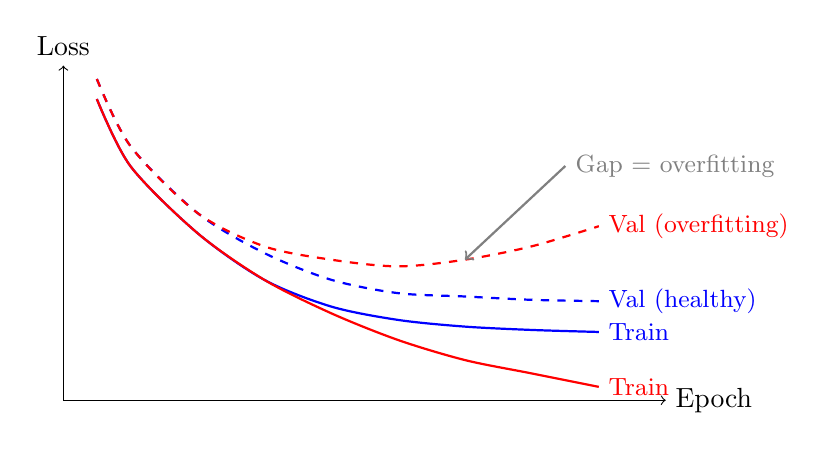
\begin{tikzpicture}[scale=0.85]
        \draw[->] (0,0) -- (9,0) node[right] {Epoch};
        \draw[->] (0,0) -- (0,5) node[above] {Loss};
        
        % Healthy training
        \draw[thick, blue] plot[smooth] coordinates {
            (0.5, 4.5) (1, 3.5) (2, 2.5) (3, 1.8) (4, 1.4) 
            (5, 1.2) (6, 1.1) (7, 1.05) (8, 1.02)
        };
        % Healthy validation
        \draw[thick, blue, dashed] plot[smooth] coordinates {
            (0.5, 4.8) (1, 3.8) (2, 2.8) (3, 2.2) (4, 1.8) 
            (5, 1.6) (6, 1.55) (7, 1.5) (8, 1.48)
        };
        
        % Overfitting
        \draw[thick, red] plot[smooth] coordinates {
            (0.5, 4.5) (1, 3.5) (2, 2.5) (3, 1.8) (4, 1.3) 
            (5, 0.9) (6, 0.6) (7, 0.4) (8, 0.2)
        };
        % Overfitting validation
        \draw[thick, red, dashed] plot[smooth] coordinates {
            (0.5, 4.8) (1, 3.8) (2, 2.8) (3, 2.3) (4, 2.1) 
            (5, 2.0) (6, 2.1) (7, 2.3) (8, 2.6)
        };
        
        % Legend
        \node[blue, right] at (8, 1.02) {\small Train};
        \node[blue, right] at (8, 1.48) {\small Val (healthy)};
        \node[red, right] at (8, 0.2) {\small Train};
        \node[red, right] at (8, 2.6) {\small Val (overfitting)};
        
        % Annotation
        \draw[<-, thick, gray] (6, 2.1) -- (7.5, 3.5) node[right, font=\small] {Gap = overfitting};
    \end{tikzpicture}
    \caption{训练损失曲线：健康训练（蓝色）vs.过拟合（红色）。实线：训练损失。虚线：验证损失。}
    \label{fig:training_curves}
\end{figure}

\subsection{梯度统计}

监控梯度统计有助于诊断训练问题：
\begin{itemize}
    \item \textbf{梯度范数：}应该稳定。尖峰表示不稳定；范数消失表示死神经元或饱和激活。
    \item \textbf{梯度分布：}应该近似高斯分布。重尾可能表示异常值样本。
    \item \textbf{更新-权重比：}比率$\|\alpha \mathbf{g}\| / \|\mathbf{W}\|$应该在$10^{-3}$左右。大得多表示不稳定；小得多表示停滞。
    \item \textbf{激活统计：}层激活的均值和方差应在整个训练过程中保持稳定。批量归一化有助于此。
\end{itemize}

\section{章节小结}

\begin{enumerate}
    \item 训练涉及对数据的迭代小批量优化，其中梯度噪声提供隐式正则化
    \item 学习率是最关键的超参数；LR范围测试提供了选择它的原则性方法
    \item 预热对于具有自适应优化器的大型模型稳定早期训练至关重要
    \item Dropout通过集成平均提供正则化，可以解释为近似贝叶斯推理
    \item AdamW将权重衰减与自适应学习率解耦，比Adam的L2正则化导致更好的泛化能力
    \item 早停防止过拟合，在某些条件下等价于正则化
    \item 混合精度训练（FP16/BF16）在正确实现时提供2-3倍加速且无精度损失
    \item 梯度累积使有效批次大小大于GPU内存的训练成为可能
    \item 系统监控损失曲线、梯度统计和验证指标对于诊断训练问题至关重要
\end{enumerate}

\section{延伸阅读}

\begin{itemize}
    \item \cite{pascanu2013difficulty} --- 训练循环神经网络的困难（梯度裁剪）
    \item \cite{srivastava2014dropout} --- Dropout：防止神经网络过拟合的简单方法
    \item \cite{goodfellow2016deep} --- 第7章（正则化）和第8章（训练深度模型的优化）
    \item \cite{gal2016dropout} --- Dropout作为贝叶斯近似：深度学习中模型不确定性的表示
    \item \cite{huang2016deep} --- 带随机深度的深度网络（随机深度）
    \item \cite{szegedy2016rethinking} --- 重新思考用于计算机视觉的Inception架构（标签平滑）
    \item \cite{goyal2017accurate} --- 准确的大批次SGD：一小时内训练ImageNet
    \item \cite{keskar2017largebatch} --- 关于大批次训练深度学习：泛化差距和尖锐最小值
    \item \cite{smith2017cyclical} --- 用于训练神经网络的循环学习率（LR范围测试）
    \item \cite{micikevicius2018mixed} --- 混合精度训练
    \item \cite{loshchilov2019decoupled} --- 解耦权重衰减正则化（AdamW）
    \item \cite{rajbhandari2020zero} --- ZeRO：面向万亿参数模型训练的内存优化
\end{itemize}

\section{练习题}

\begin{enumerate}
    \item \textbf{学习率范围测试：}描述您将如何运行LR范围测试并解释损失曲线以选择初始学习率。

    \item \textbf{预热原理：}为什么预热对于大批次训练和Transformer优化特别重要？它防止什么失败模式？

    \item \textbf{权重衰减：}在自适应优化器背景下比较L2正则化和AdamW。为什么两者可能表现不同？

    \item \textbf{早停：}解释为什么早停可以被视为一种正则化形式。什么验证模式表明应该停止训练？

    \item \textbf{混合精度：}如果FP16使激活内存减半，通常添加什么次要机制来保持梯度数值稳定？

    \item \textbf{梯度累积：}假设您可以在一块GPU上容纳批次大小16，但需要有效批次大小128。需要多少累积步数，调用backward前应该对损失做什么？
\end{enumerate}
